\documentclass{article}

% Packages
\usepackage{titling}
\usepackage[utf8]{inputenc}
\usepackage[english]{babel}
\usepackage{amsmath,amssymb}
\usepackage{graphicx}
\usepackage{float}
\usepackage{subcaption}
\usepackage[hidelinks]{hyperref}
\usepackage{listings}
\usepackage[a4paper, top = 2cm, bottom = 2cm, left = 2cm, right = 2cm, footskip=0.8cm]{geometry}
\usepackage{multicol}
\usepackage{booktabs}
\usepackage{array}
\usepackage[table]{xcolor}
\usepackage{geometry}% Package for margin adjusting
\usepackage{titlesec} % Package to change title format
\usepackage{enumitem}
\usepackage{algorithm}
\usepackage{algorithmic}
\usepackage{multirow}
\usepackage{comment}

\definecolor{pyblue}{RGB}{31,119,240}

\geometry{
  left=2cm, % adjust the left margin
  right=2cm, % adjust the right margin
  top=2cm, % adjust the top margin
  bottom=2cm, % adjust the bottom margin
}

\titlespacing*{\subsection}{0pt}{10pt}{7pt}
\titlespacing*{\section}{0pt}{10pt}{4pt}



\graphicspath{{Figures/}}
\newcolumntype{M}[1]{>{\centering\arraybackslash}m{#1}}



% Title page information
\pretitle{
  \begin{center}
  \LARGE
  \vspace{-0.9cm}
  
\includegraphics[width=15.1cm,height=3.05cm]{Logo_unipv.png}\vspace*{0.6cm}\\[\bigskipamount]}


\title{\Large Machine Learning Course\vspace{0.4cm}\\
    \rule{\textwidth}{0.3pt}\vspace{0.3cm}\\
    \textbf{I'm Not Clickbaiting You... It's a Headline, I Swear!}\vspace{0.2cm}\\
    \large{A machine learning solution against clickbait}
    \rule{\textwidth}{0.3pt}\vspace{0.5cm}}

\posttitle{\end{center}}
    
\author{Andrea Alberti\vspace{0.2cm}\\
    \small Department of Computer Engineering - Data Science\\[0.2cm]
    \small University of Pavia, Italy \\
    \small Email: andrea.alberti01@universitadipavia.it \\
    \small GitHub: \href{https://github.com/AndreaAlberti07/Clickbait-Detection-ML.git}{\underline{https://github.com/AndreaAlberti07/Clickbait-Detection-ML.git}}\vspace{0.5cm}}
        
\date{\today}

\begin{document}

\begin{titlepage}
   
        \maketitle
        \thispagestyle{empty}

    \begin{multicols*}{2}
            
        \hrule
        \begin{abstract}
        \noindent
        This report explores the implementation of classification algorithms for clickbait detection, with a focus on comparing the 
        performance of the Multinomial Naïve Bayes Classifier and Logistic Regression models. The objective of the project is to 
        evaluate the effectiveness of these models in identifying clickbait content using two different approaches: an accuracy-oriented 
        approach and an approach targeting the minimization of False Positive Rate (FPR).

        The experimentation of various combinations of vocabulary size and type, led to the selection of models that demonstrate impressive 
        results. In the accuracy-oriented scenario, the models achieved a test accuracy of 97.12\%. In the FPR-oriented scenario, a 0\% FPR was 
        achieved on the test set, while maintaining a good accuracy of 84\%.

        Additionally, this project provides valuable information about the composition of clickbait headlines. It identifies the most impactful 
        words for the classification models, shedding light on the characteristics that make headlines challenging to classify accurately. 
        The analysis of the worst errors further enhances the understanding of the limitations of the model.
        \\
        \end{abstract}
     \newcolumn
        \hrule
        \tableofcontents
    \end{multicols*}

\end{titlepage}

\newpage
\pagenumbering{arabic}



%---------------------------------------------------------

\begin{multicols}{2}
    
\section{Introduction}
Clickbait headlines have inundated the digital landscape, flashing users with sensational promises and generating significant challenges 
for content consumers and platforms. To address this issue, classification algorithms have emerged as a solution for identifying clickbait 
content automatically. This report explores the implementation of these algorithms, comparing their effectiveness and performance. 
By understanding clickbait detection advancements, it is possible to tackle the issue of misleading headlines and improve the reliability of online information.

%-----------------------------------------------------------

\section{Goal}
The objective of this project is to train and compare the performance of the \textit{Multinomial Naïve Bayes Classifier} and \textit{Logistic Regression} 
in clickbait detection. The project focuses on two scenarios: the first is an accuracy-oriented approach, aiming to maximize the classifier's overall accuracy. 
The second scenario is FPR-oriented, prioritizing the minimization of False Positive Rate (FPR) while maintaining a satisfactory level of accuracy.

%-----------------------------------------------------------

\section{Data}
The data consists of a dataset of 32,000 headlines. The dataset is evenly divided into two classes: 'clickbait' and 'non-clickbait'. 
It comprises three subsets: training, validation, and test sets, containing 24,000, 4,000, and 4,000 samples, respectively.
The data is stored in text files, with one headline for each line.

\subsection{Data Pre-processing}
To prepare the data for the algorithms it is necessary to convert the headlines into a numerical representation (features extraction). 
One common way tor this is to create the \textit{Bag of Words} representation. This process involves two steps:

\vspace{-0.20cm}
\begin{itemize}[leftmargin=9pt]
\item \textbf{Build a vocabulary}: the vocabulary is a sub-list of all the words that appear in the training set.\vspace{-0.1cm}
\item \textbf{Build the BoW}: each headline is represented as a vector of length equal to the vocabulary size. Each element of the vector is the 
number of times the corresponding word appears in the headline.
\end{itemize}\vspace{-0.25cm}

For this project two types of vocabulary were created: one with stopwords removed and one without, each one with different sizes.
The punctuation was removed, but the numbers were kept.

%-----------------------------------------------------------

\section{Classification Models}
The two used models follow different philosophies. The Naïve Bayes Classifier is a generative model, while Logistic Regression is a discriminative one.

\subsection{Multinomial Naïve Bayes}
As a generative model, it classifies data by first learning $P(Y=y)$ and $P(X=j|Y=y) = \pi_{y,j}$ independently for each class $y$. Specifically, it assumes
a multinomial distribution for $P(X|Y=y)$, thereby it classifies according to the following rule: 

\vspace{-0.2cm}
\begin{equation}
    \hat{y} = arg\max_y \sum_{j=0}^{n-1} x_j \log{\pi_{y,j}} + \log{P(Y)} 
\end{equation}
\vspace{-0.5cm}

\subsection{Logistic Regression}
As a discriminative model, it classifies data by learning the boundary directly. Specifically, it learns the function \ref{eq:funct} and estimates 
$P(Y=1|X=\mathbf{x_i})$ as \ref{eq:prob}. 

\vspace{-0.2cm}
\begin{equation} \label{eq:funct}
    z_i = b_i + w_1x_{i1} + w_2x_{i2} + .... + w_nx_{in}
\end{equation}
\vspace{-0.2cm}
\begin{equation} \label{eq:prob}
    \hat{p_i}=\frac {1}{1+e^{-z_i}}
\end{equation}
\vspace{-0.65cm}

%-----------------------------------------------------------

\section{Scenarios}

The primary concern in certain use cases may not always be the overall accuracy of the model, but rather minimizing the number of false positives. 
For instance, in clickbait detection, misclassifying legitimate headlines as clickbait can lead to user frustration. 
Thus, it is important to prioritize reducing the number of false positives. 
Indeed accuracy remains important, therefore a reasonable tradeoff needs to be found.
In this project, for each scenario, the two models were trained and evaluated using
different sizes of the two vocabulary types (with and without stopwords).

\subsection{Max Accuracy Oriented}
The results of this scenario are summarized in Figure \ref{ACC_all}, where the model accuracies are compared changing vocabulary size and type.

    \begin{figure}[H]
        \centering
        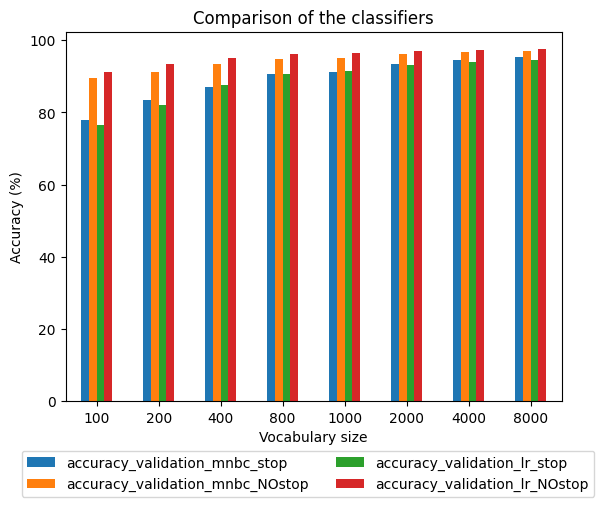
\includegraphics[width=1\columnwidth]{Figures/ACC_all.png}
        \caption{\footnotesize Accuracy for all models}
        \label{ACC_all}
    \end{figure}

A first outcome is about the \textbf{vocabulary type}. The models trained with the vocabulary without stopwords ('\_stop') perform worse than the ones trained 
with the vocabulary with stopwords ('\_NOstop'). This indicates that these latter may be useful. Moreover, it is worth to underline that each headline is made up 
by only a few words, therefore removing stopwords may lead to a loss of information.
A second results is about the \textbf{vocabulary size}. In general, there is a positive correlation between the size of the vocabulary and the 
validation accuracy. As the vocabulary size increases, the model's ability to capture a wider range of linguistic patterns and variations 
improves, as witnessed by Figure \ref{fig:ROC}. However, it's important to note that this correlation tends to plateau after a certain dimension.\\
Regarding the \textbf{model type}, both the Multinomial Naïve Bayes Classifier and Logistic Regression models demonstrate similar performance. 
However, the Logistic Regression model requires more time to train due to the optimization process and hyperparameters choice\footnotemark. Consequently, the Naïve Bayes Classifier 
is preferred due to its faster training time, allowing for selecting the model with the largest vocabulary size.
Finally, its efficient training time, coupled with the validation accuracy of 97\% make the NBC with stopwords and vocabulary size 
of 8000 the best model for this scenario.

        \footnotetext{The details about the Logistic Regression setup are reported in section \ref{sec:LR_details}}

\subsection{Min FPR Oriented}
To find the model with the lowest FPR, the biases were varied in the range [-8, 8] for LR and [5, -5 ; -5, 5] for MNBC.
Subsequently the algorithm \ref{alg:1} was appositely developed and applied.


\begin{algorithm}[H]
    \small
    \caption{Finding the Model with the Lowest FPR}
    \begin{algorithmic}[1]
    \FOR{each Model}
    \FOR{each Vocabulary Type}
    \FOR{each Size in Vocabulary Sizes}
    \FOR{each $b'$ in biases}
    \STATE Train Model $\rightarrow$ $w, b$
    \STATE $w, b' \rightarrow$ Make Inference on Validation
    \STATE Compute FPR
    \ENDFOR
    \STATE Take smallest FPR, related $b'$ and accs
    \ENDFOR
    \ENDFOR
    \ENDFOR
    \end{algorithmic}
    \label{alg:1}
    \end{algorithm}
  

\noindent
The results are presented in Figure \ref{fig:MNBC} and Figure \ref{fig:LR}. 
Once again, it is evident that the models that do not remove stopwords (bottom chart in the figures) outperform the others, limiting our choice to these models.
Both the MNBC and LR models exhibit impressive performance, 
achieving an FPR of 0.0005 (0.05\%) while maintaining a high accuracy above 84\%. 
While some instances show a 0\% FPR, it is important to note that these results may vary with small changes in the test set, therefore
a difference of 0.05\% is not considered significant.
Considering the aforementioned advantages of fast training and the favorable trade-off between accuracy and fpr, the \textbf{MNBC with a vocsize of 2000} 
is chosen as the best model. Note that by picking another bias\footnotemark, the model can be tailored to the specific case.


    \begin{figure}[H]
        \begin{subfigure}{\linewidth}
        \centering
        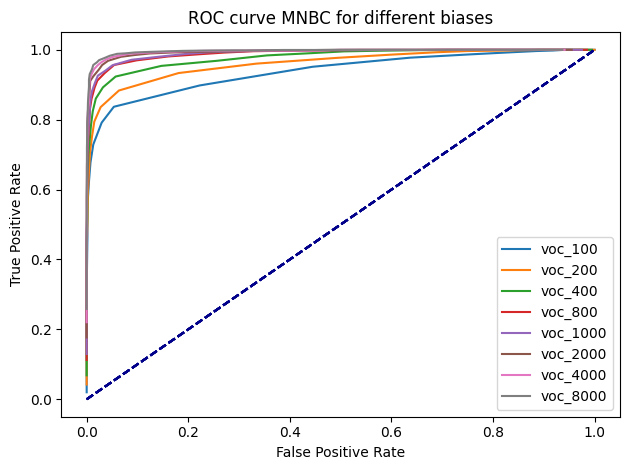
\includegraphics[width=0.87\columnwidth]{Figures/ROC_mnbc_nostop.png}
        \end{subfigure}
        
        \begin{subfigure}{\linewidth}
        \centering
        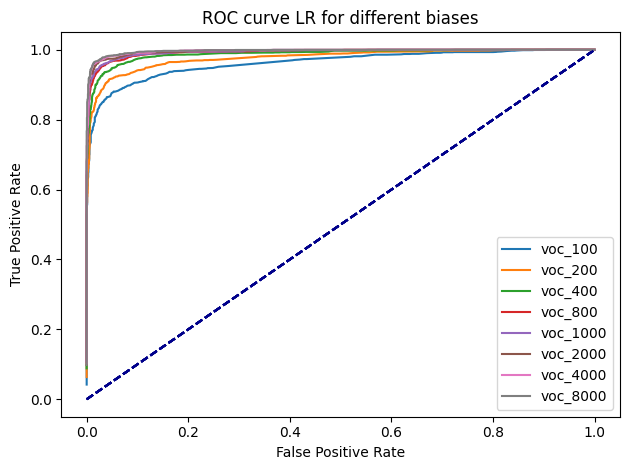
\includegraphics[width=0.87\columnwidth]{Figures/ROC_lr_nostop.png}
        \end{subfigure}
        
        \caption{\footnotesize ROC curves for models keeping stopwords}
        \label{fig:ROC}
    \end{figure}    

    \begin{figure}[H]
        \begin{subfigure}{\linewidth}
        \centering
        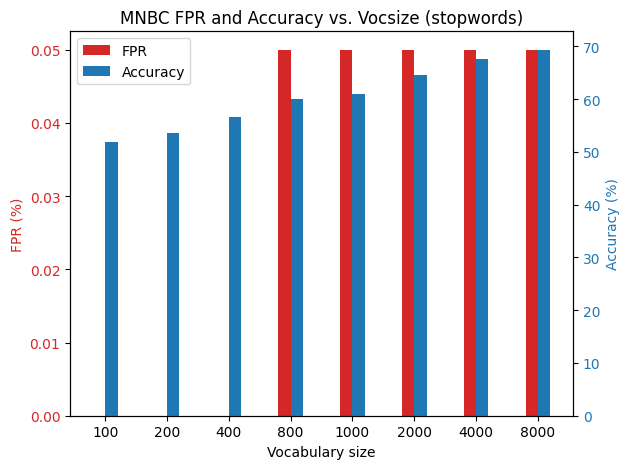
\includegraphics[width=0.96\columnwidth]{Figures/FPR_mnbc_stop.png}
        \end{subfigure}
        
        \begin{subfigure}{\linewidth}
        \centering
        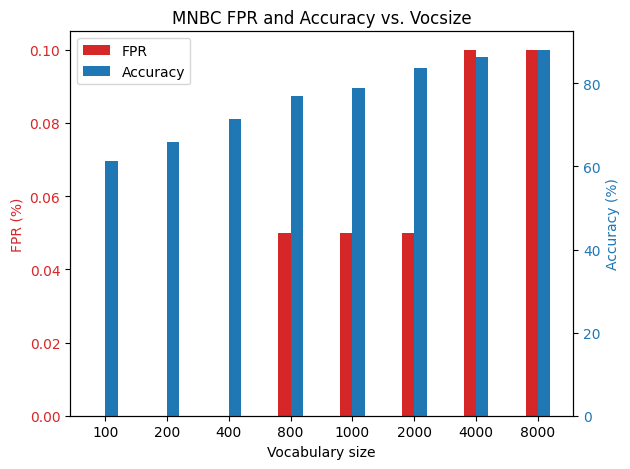
\includegraphics[width=0.96\columnwidth]{Figures/FPR_mnbc_nostop.png}
        \end{subfigure}
        
        \caption{\footnotesize FPR and validation\_accs for MNBC}
        \label{fig:MNBC}
    \end{figure}

    \begin{figure}[H]
        \begin{subfigure}{\linewidth}
        \centering
        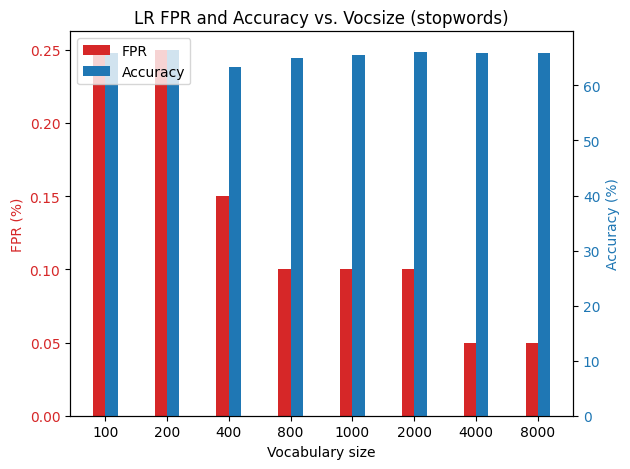
\includegraphics[width=0.97\columnwidth]{Figures/FPR_lr_stop.png}
        \end{subfigure}
        
        \begin{subfigure}{\linewidth}
        \centering
        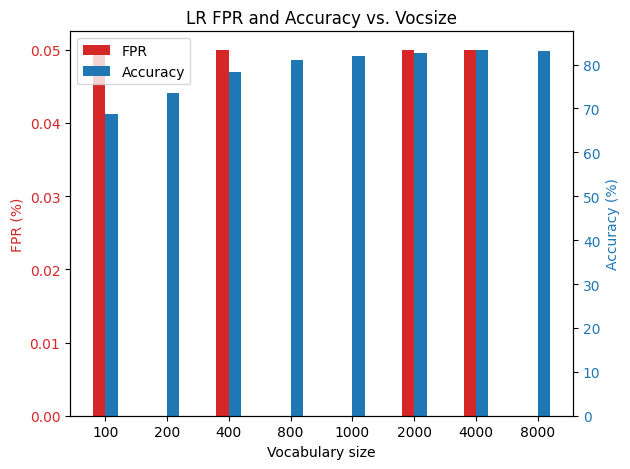
\includegraphics[width=0.97\columnwidth]{Figures/FPR_lr_nostop.png}
        \end{subfigure}
        
        \caption{\footnotesize FPR and validation\_accs for LR}
        \label{fig:LR}
    \end{figure}
  
\noindent
The results of the best model are summarized in Table \ref{tab:best_model_lr}.


    \begin{table}[H]
        \small
        \centering
        \rowcolors{2}{pyblue!25}{white}
        \begin{tabular}{|c|c|c|c|c|}
        \hline
        \rowcolor{pyblue!60}
        \textbf{Vocsize} & \textbf{biases} & \textbf{FPR} & \textbf{TPR} & \textbf{Val\_acc} \\ \hline
        2000 & 5,-5 & 0.0005 & 0.672 & 83.58\% \\ \hline
        \end{tabular}
        \caption{\footnotesize Best Model FPR scenario}
        \label{tab:best_model_lr}
    \end{table}

%-----------------------------------------------------------
    
\section{Best Models Analysis}
Based on the previous sections, the best model have been identified for each scenario are:

        \footnotetext{Further results available at \href{https://github.com/AndreaAlberti07/Clickbait-Detection-ML.git}{\underline{this GitHub}} repository}


    \begin{itemize}[leftmargin=9pt]
        \item \textbf{Max Accuracy Oriented}: MNBC with stopwords kept and vocabulary size of 8000
        \item \textbf{Min FPR Oriented}: MNBC with stopwords kept, vocabulary size of 2000 and biases = [5, -5]
    \end{itemize}

\noindent
In this section, a comprehensive analysis of the best models is presented, including an investigation into their 
worst errors and the identification of the most impactful words on the test set.

    \begin{itemize}[leftmargin=9pt]
        \item \textbf{Most impactful words}: the most impactful words for a class are those that most influence the classification score in favour of that class. They are taken looking at the probability
        gap of each word between the two classes.
        \item \textbf{Worst errors}: these are the data misclassified with the higher confidence. In other words, are the headlines for which the gap between the
        classification scores of the two classes is the largest.
    \end{itemize}
\noindent
Finally, the models are evaluated on the test set, and the results are documented.

\subsection{Max Accuracy Oriented}

\textbf{Most impactful words}\\
The results are reported in Table \ref{tab:MIW_acc_scenario}. 
The words in the "Bait" column, with their negative deltas, have been determined to be strongly associated with clickbait headlines. 
These words may include terms commonly used in clickbait headlines, such as specific years ('2015'), attention-grabbing phrases 
('hilarious'), or words that provoke curiosity or emotional engagement ('guess'). When these words appear in a headline, they 
tend to increase the likelihood of it being classified as clickbait.
On the other hand, the words in the 'Nobait' column, with their positive deltas, are associated with non-clickbait headlines. 
These words may include terms related to news topics ('iraq', 'afghanistan'), informative language ('announces'), or general topics 
of interest ('nuclear'). When these words are present in a headline, they tend to decrease the likelihood of it being classified 
as clickbait.
The model learned 
to assign weights and deltas to words based on their frequency and association with clickbait or non-clickbait labels in the 
training data. Through this process, the model identified these impactful words as important features that contribute significantly 
to the classification decision.

    \begin{table}[H]
        \small
        \centering
        \rowcolors{2}{pyblue!25}{white}
        
        \begin{tabular}{|c|c|c|c|}
        \hline
        \rowcolor{pyblue!60}
        \textbf{Bait} & \textbf{Delta} & \textbf{Nobait} & \textbf{Delta}\\ \hline
        2015 & -5.70 & kills & 5.56 \\ \hline
        things & -5.69 & iraq & 5.36 \\ \hline
        these & -5.24 & wins & 4.88 \\ \hline
        tweets & -5.02 & afghanistan & 4.88 \\ \hline
        you & -5.01 & leader & 4.85 \\ \hline
        guess & -4.97 & wikinews & 4.68 \\ \hline
        hilarious & -4.76 & announces & 4.64 \\ \hline
        actually & -4.76 & zealand & 4.59 \\ \hline
        ve & -4.62 & nuclear & 4.58 \\ \hline
        instagram & -4.57 & iraqi & 4.55 \\ \hline
        \end{tabular}
        \caption{\footnotesize Most impactful words for the best ACC scenario}
        \label{tab:MIW_acc_scenario}
    \end{table}


\noindent
\textbf{Worst errors} \\
In Figure \ref{fig:WE_ACC} are shown respectively the false positives and the false negatives
on the test set, together with the headlines content and the model confidence. The misclassified headlines seems reasonable, since even a 
human could have some doubts about their classification. Despite the length of the headlines might appear as an influencing factor, as the 
false positives are shorter than the false negatives, it is not the case as depicted in Table \ref{tab:LENGTH_acc}. This analysis is useful
to provide information about how, the headlines capable of deceiving the model, are composed.

    \begin{figure}[H]
        
        \begin{subfigure}{\linewidth}
        \centering
        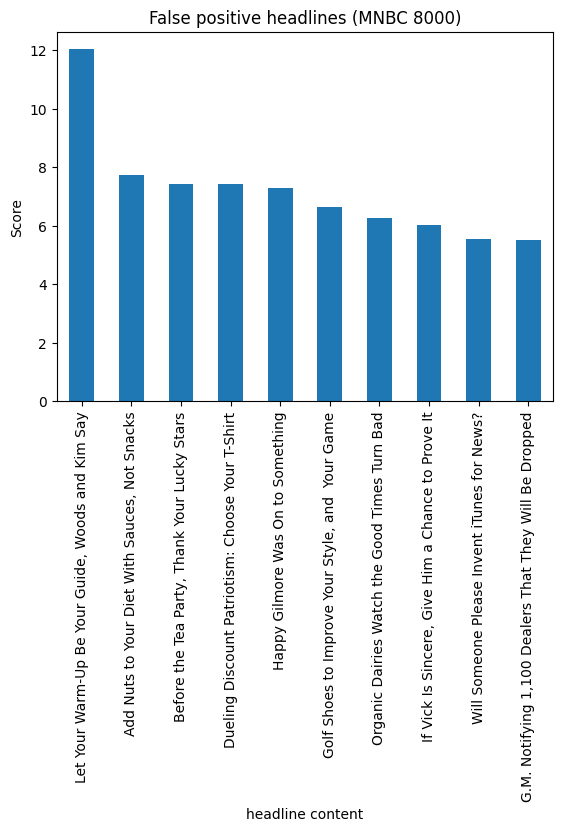
\includegraphics[width=0.90\columnwidth]{Figures/false_pos_bestACC.png}
        \end{subfigure}
        
        \begin{subfigure}{\linewidth}
        \centering
        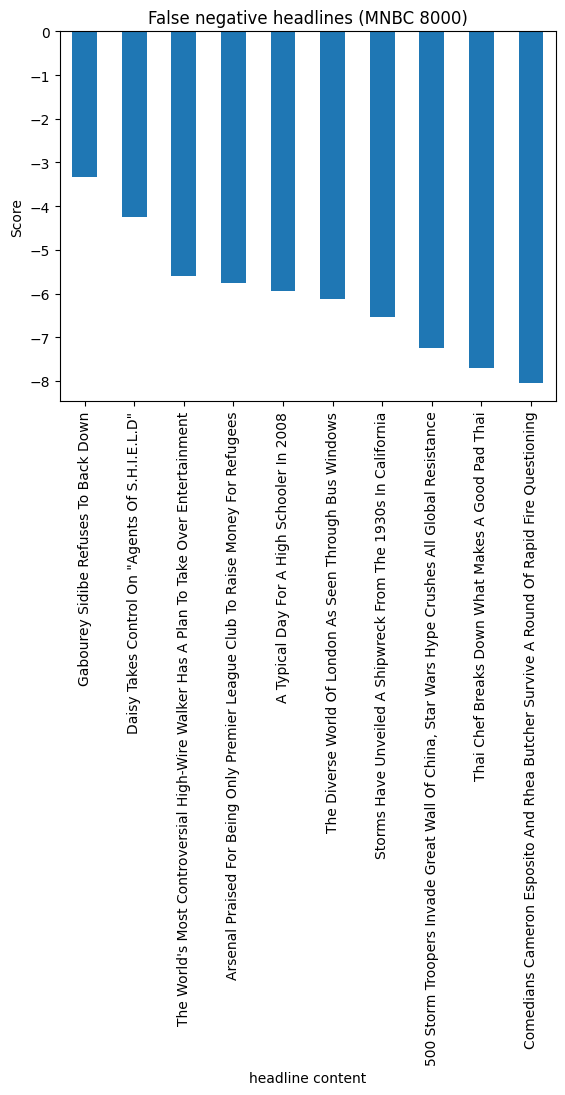
\includegraphics[width=0.90\columnwidth]{Figures/false_neg_bestACC.png}
        \end{subfigure}
        
        \caption{\footnotesize Worst errors for MNBC (8000)}
        \label{fig:WE_ACC}
        
    \end{figure}

\begin{table}[H]
    \small
    \centering
    \rowcolors{2}{pyblue!25}{white}
    \begin{tabular}{|c|c|c|}
    \hline
    \rowcolor{pyblue!60}
    \textbf{Misclassified} & \textbf{All} & \textbf{Correctly Classified}\\ \hline
    8.65 & 9.11 & 9.12 \\ \hline
    \end{tabular}
    \caption{\footnotesize Avg length (n. words) of the headlines}
    \label{tab:LENGTH_acc}
\end{table}

\noindent
\textbf{Results on Test set}\\
The results reported in Table \ref{tab:test_acc_scenario} confirm the impressive performance of the model,
achieving a test accuracy of 97.12\% despite its simplicity.

    \begin{table}[H]
        \small
        \centering
        \rowcolors{2}{pyblue!25}{white}
        \begin{tabular}{|c|c|}
        \hline
        \rowcolor{pyblue!60}
        \textbf{Train Accuracy} & \textbf{Test Accuracy} \\ \hline
        97.88\% & 97.12\% \\ \hline
        \end{tabular}
        \caption{\footnotesize Test results for the best ACC scenario}
        \label{tab:test_acc_scenario}
    \end{table}



\subsection{Min FPR Oriented}

\textbf{Most impactful words}\\
The most impactful words for this scenario are reported in Table \ref{tab:MIW_fpr_scenario}. It is interesting to note that the words
are the same as the ones for the best accuracy scenario, with slightly different deltas. 
This indicates the robustness of these features in identifying clickbait headlines. 
Specifically, it suggests that these words carry substantial information about the clickbait 
nature of the headlines and can serve as reliable indicators for classification purposes.

\begin{table}[H]
    \small
    \centering
    \rowcolors{2}{pyblue!25}{white}
    
    \begin{tabular}{|c|c|c|c|}
    \hline
    \rowcolor{pyblue!60}
    \textbf{Bait} & \textbf{Delta} & \textbf{Nobait} & \textbf{Delta}\\ \hline
    2015 & -5.54 & kills & 5.72 \\ \hline
    things & -5.53 & iraq & 5.52 \\ \hline
    these & -5.08 & afghanistan & 5.04 \\ \hline
    tweets & -4.86 & wins & 5.04 \\ \hline
    you & -4.84 & leader & 5.01 \\ \hline
    guess & -4.81 & wikinews & 4.84 \\ \hline
    hilarious & -4.60 & announces & 4.80 \\ \hline
    actually & -4.60 & zealand & 4.75 \\ \hline
    ve & -4.46 & nuclear & 4.74 \\ \hline
    instagram & -4.41 & iraqi & 4.71 \\ \hline
    \end{tabular}
    \caption{\footnotesize Most impactful words for the lowest FPR scenario}
    \label{tab:MIW_fpr_scenario}
    \end{table}

\noindent
\textbf{Worst errors} \\
\noindent
In the analysis of the worst errors, the false negatives are not reported since they are the same as those for the 
best accuracy scenario. Moreover, it is noticeable that the model did not produce any false positives on 
the test set. This outcome highlights the effectiveness of the model in minimizing the False Positive Rate 
(FPR). According to Table \ref{tab:low_fpr_scenario} the TPR is 68\% which means that the model is able both to
avoid false positives and recalling 7 out of 10 clickbait headlines.

It is worth mentioning that the relation between FPR and TPR is expressed by the ROC curve and can be tuned
at any time by changing the bias, tailoring the model to the specific use case.
\\

\noindent
\textbf{Results on Test set}\\
The results reported in Table \ref{tab:low_fpr_scenario} confirm the excellent performance of the model,
achieving a False Positive Rate of 0\% on the test set.

    \begin{table}[H]
        \small
        \centering
        \rowcolors{2}{pyblue!25}{white}
        \begin{tabular}{|c|c|c|}
        \hline
        \rowcolor{pyblue!60}
        \textbf{Test Accuracy} & \textbf{FPR} & \textbf{TPR}\\ \hline
        84.00\% & 0.0\% & 68\%\\ \hline
        \end{tabular}
        \caption{\footnotesize Test results for the lowest FPR scenario}
        \label{tab:low_fpr_scenario}
    \end{table}


%-----------------------------------------------------------


\section{Details: Logistic Regression}\label{sec:LR_details}
In this section a brief overview about the Logistic Regression setup is provided.\\
All the results in the previous sections were obtained training the model using the full batch gradient 
descent algorithm, with a learning rate of 0.001 and 1000 iterations. No regularization was applied.\\
The training was limited to 1000 iterations since a convergence trend was observed in the loss function. 
This decision was made to strike a balance between ensuring convergence and allowing for the exploration of multiple 
scenarios within a reasonable training time frame.\\
The learning rate was selected from a range of options, including 0.0001, 0.0003, 0.001, 0.003, 0.01, 0.03, and 0.1. 
The choice was guided by observing the behavior of the loss function during training, specifically looking for a 
steep and consistent decreasing trend without oscillations.\\
Since the model did not exhibit overfitting, displaying a small discrepancy between the training and validation 
accuracy, no regularization techniques were employed.\\

\noindent
For seek of completeness the LR with a vocabulary size of 4000 and keeping stopwords, was trained using the
following specifications:

    \begin{itemize}[leftmargin=9pt]
        \item \textbf{Learning rate}: 0.001
        \item \textbf{Iterations}: 20000 
        \item \textbf{Regularization}: 0.2
        \item \textbf{Tolerance}: 0.0000005
    \end{itemize}

\noindent
Looking at the results depicted in Figure \ref{fig:ACC_lr_deep} and Figure \ref{LOSS_lr_deep}, they are evident both
the convergence of the model after few iterations and the small gap between the training and validation accuracy.

    \begin{figure}[H]
        \centering
        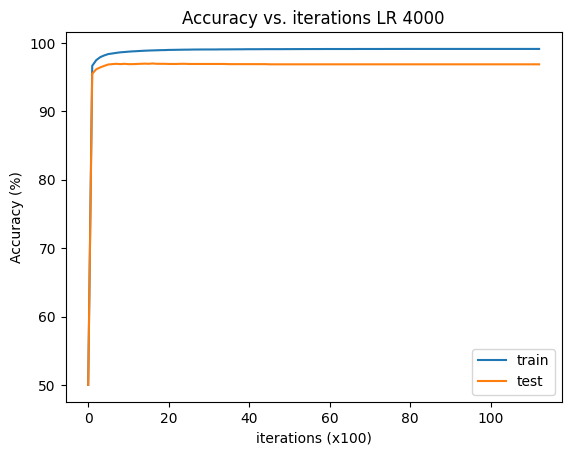
\includegraphics[width=0.9\columnwidth]{Figures/ACC_lr_deep.png}
        \caption{\footnotesize Accuracy for LR}
        \label{fig:ACC_lr_deep}
    \end{figure}

    \begin{figure}[H]
        \centering
        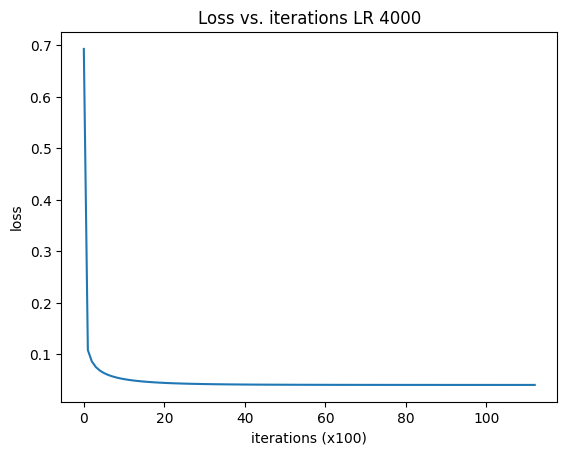
\includegraphics[width=0.9\columnwidth]{Figures/LOSS_lr_deep.png}
        \caption{\footnotesize Loss function for LR }
        \label{LOSS_lr_deep}
    \end{figure}


%-----------------------------------------------------------

\section{Conclusions and Future Work}
\textbf{Future Work}\\
The inclusion of numbers in the vocabulary is important for the clickbait classification model as clickbait headlines 
often contain numeric values. However, in the list of impactful words, can be noticed that only one number appears.
This is because the model relies solely on the frequency of a specific word in the clickbait and 
non-clickbait classes, without recognizing whether a word is specifically a number or not. Since headlines 
can include a wide range of different numbers, the model is unable to identify a specific number as impactful.
Adding a feature to identify numbers in headlines could significantly enhance the already good model's performance.\\

\noindent
\textbf{Conclusions}\\
In summary, the outcomes obtained in this project can be deemed satisfactory. Remarkable performance was 
observed in both scenarios for the tested models. Among them, the Multinomial Naïve Bayes Classifier emerged 
as the preferred choice due to its ability to deliver notable results with minimal training efforts. 
The composition of the vocabulary was identified as a crucial element in influencing the model's performance, 
with the inclusion of stopwords yielding superior outcomes. Additionally, the results underscored the significance 
of vocabulary size, indicating that larger vocabularies correlate with improved performance.\\
Lastly, the project offered information about the structure of headlines capable of fooling the model, 
and revealed that attention-grabbing and emotionally engaging words are commonly used for clickbait headlines.

\noindent
The code and further results of this project can be freely accessed and reviewed on the GitHub repository at 
\href{https://github.com/AndreaAlberti07/Clickbait-Detection-ML.git}{\underline{AndreaAlberti07/Clickbait-Detection-ML.git}}.\\


%-----------------------------------------------------------



%\nopagebreak

%\vfill
%\noindent
%\textcolor{gray!80}{\textbf{Declaration}}\\
%\textcolor{gray!70}{I affirm that this report is the result of my own work and that I did not share any part of it with anyone else except the teacher.
%}


\end{multicols}
\end{document}


\begin{comment}

TABLES SUMMARIZING SOME OF THE FPR RESULTS

\begin{table}[H]
    \small
    \centering
    \rowcolors{2}{pyblue!25}{white}
    
    \begin{tabular}{|c|c|c|c|c|}
    \hline
    \rowcolor{pyblue!60}
    \textbf{Vocsize} & \textbf{Bias} & \textbf{FPR \%} & \textbf{TPR \%} & \textbf{Acc \%} \\ \hline
    1000 & -8.0 & 0.0005 & 0.718 & 85.88 \\ \hline
    2000 & -8.0 & 0.001 & 0.733 & 86.6 \\ \hline
    4000 & -8.0 & 0.001 & 0.7465 & 87.28 \\ \hline
    8000 & -8.0 & 0.0 & 0.7465 & 87.32 \\ \hline
    1000 & -7.0 & 0.0025 & 0.7875 & 89.25 \\ \hline
    2000 & -7.0 & 0.002 & 0.8095 & 90.38 \\ \hline
    4000 & -7.0 & 0.003 & 0.8175 & 90.72 \\ \hline
    8000 & -7.0 & 0.001 & 0.8215 & 91.02 \\ \hline
    \end{tabular}
    \caption{\footnotesize FPR results for Logistic Regression}
    \label{tab:fpr_results_lr}
\end{table}

\begin{table}[H]
    \small
    \centering
    \rowcolors{2}{pyblue!25}{white}
    \begin{tabular}{|c|c|c|c|c|c|}
    \hline
    \rowcolor{pyblue!60}
    \textbf{Vocsize} & \textbf{Biases} & \textbf{FPR \%} & \textbf{TPR \%} & \textbf{Acc \%} \\ \hline
    1000 & 5.0, -5.0 & 0.0005 & 0.5805 & 79.0 \\ \hline
    2000 & 5.0, -5.0 & 0.0005 & 0.672 & 83.58 \\ \hline
    4000 & 5.0, -5.0 & 0.001 & 0.727 & 86.3 \\ \hline
    8000 & 5.0, -5.0 & 0.001 & 0.7635 & 88.12 \\ \hline
    1000 & 4.0, -4.0 & 0.0015 & 0.697 & 84.78 \\ \hline
    2000 & 4.0, -4.0 & 0.0015 & 0.7665 & 88.25 \\ \hline
    4000 & 4.0, -4.0 & 0.002 & 0.8095 & 90.38 \\ \hline
    8000 & 4.0, -4.0 & 0.002 & 0.8415 & 91.98 \\ \hline
    \end{tabular}
    \caption{\footnotesize FPR results for Multinomial NBC}
    \label{tab:fpr_results_mnbc}
\end{table}

\end{comment}